% !TeX root = RJwrapper.tex
  
  \title{Resampling Fuzzy Numbers with Statistical Applications: \pkg{FuzzyResampling} Package}
  \author{by Maciej Romaniuk, Przemys{\l}aw Grzegorzewski}
  
  \maketitle
  
\abstract{
  The classical bootstrap has proven its usefulness in many areas of statistical inference.
  However, some shortcomings of this method are also known.
  Therefore, various bootstrap modifications and other resampling algorithms have been introduced, especially for real-valued data.
  Recently, bootstrap methods have become popular in statistical reasoning based on imprecise data often modeled by fuzzy numbers.
  One of the challenges faced there is to create bootstrap samples of fuzzy numbers which are similar to initial fuzzy samples but different in some way at the same time.
  These methods are implemented in \CRANpkg{FuzzyResampling} package and applied in different statistical functions like single-sample or two-sample tests for the mean.
  Besides describing the aforementioned functions, some examples of their applications as well as numerical comparisons of the classical bootstrap with the new resampling algorithms are provided in this contribution.
  }
  
%%%%%%%%%%%%%%%%%%%%%%%%%%%%%%%%%%%%%%%%%%%%%%%%%%%


\section{Introduction} 

The bootstrap introduced by \cite{Efron} is one of the most important contemporary achievements of computational statistics. 
It has proven its usefulness in various fields, e.g., in estimating standard errors, computing confidence intervals, or hypothesis testing, especially if the actual population  distribution is unknown or the desired statistical procedures are not tractable analytically, and when the sample size is not large enough to apply asymptotic methods (e.g, \cite{EfroTibs93}). Then \cite{gine} developed a bootstrapped approximation to the Central Limit Theorem for generalized random elements, which allows to apply bootstrap for fuzzy random variables used for modeling imprecise outputs of random experiments. This application is of extreme importance because the absence of suitable models for the distribution of fuzzy random variables makes the statistical reasoning difficult. Practice has shown that the use of the bootstrap to handle fuzzy data has been very effective (e.g., \cite{gil,gonzalezrodriguez,montenegro2004,LUBIANO2016918,LUBIANO2017128}).

An important disadvantage of the classical bootstrap, easily spotted especially for small sample sizes, is that the bootstrap samples almost always contain repeated values and hence their variability is lower when compared to the initial sample.
This is more troublesome when the random distribution of the assumed statistical model is continuous, since this feature is not properly reflected with the classical bootstrap where each value has the same non-zero probability of appearing in the bootstrap sample. To overcome this problem many modifications of Efron's approach were proposed in the literature, like the smoothed bootstrap \citep{Silverman}. 
The same shortcomings and remarks apply to bootstrap methods applied in a fuzzy environment. Here it would also be desirable to generate samples consisting of fuzzy observations that are almost identical to those contained in the original sample, but nevertheless different from them to some extent. 
Several methods have been proposed to deal with this problem \citep{GrzegorzewskiRom2021}. One can divide them into two main groups. The first one group shares the generation of new fuzzy numbers which keep some ``characteristic points'' of the membership functions describing initial fuzzy values. 
For the second group, we are interested in the preservation of some basic characteristics of the initial values, like their canonical representation \citep{delgado}.
Both approaches seem to be fruitful in many aspects of the statistical inference (see \cite{grzegorzewski2019,grzegorzewski_ijcis2020,grzegorzewski_amcs2020,GrzegorzewskiRom2021,romaniuk2019,romaniuk_hryniewicz}) and may be helpful in improving the results
of some real-life data analyses.

To allow potential users access to the aforementioned new bootstrap methods, several resampling algorithms have been implemented in \CRANpkg{FuzzyResampling} package \citep{FuzzyResamplingMan}. They have been complemented by some additional procedures which might be useful for the generation of samples of trapezoidal fuzzy numbers, for estimation of the standard error (or the MSE), and for testing hypotheses about the fuzzy mean (in the single or two samples problem), etc. 
The proposed package can be applied together with other tools designed for data analysis.
\pkg{FuzzyResampling} is, to our knowledge, the first package in R \citep{RMan} which provides a few resampling methods for trapezoidal fuzzy numbers together with some statistical functions based on them.

In the following, we briefly compare \pkg{FuzzyResampling} with the existing packages, introduce a necessary notation and describe the new resampling methods.
Functions implemented in the package are illustrated with examples.
Finally, the proposed resampling methods are compared with the classical bootstrap in some important statistical problems (both theoretical and utilizing real-life data).



%%%%%%%%%%%%%%%%%%%%%%%%%%%%%%%%%%%%%%%%%%%%%%%%%%%


\subsection{Related packages}

There is an abundance of packages oriented toward the classic bootstrap and its statistical applications, like \CRANpkg{boot} \citep{bootMan}, with many functions and data originated from \cite{davison_hinkley_1997} including the parametric and nonparametric resampling approaches, or \CRANpkg{bootstrap} \citep{bootstrapMan}, which contains functions and data related to \cite{EfroTibs93}, e.g. cross-validation or jackknife procedures.

There are also many R packages intended to handle fuzzy numbers that may be useful in statistical reasoning with fuzzy data.
Researchers can utilize  \CRANpkg{FuzzyNumbers} \citep{FuzzyNumbersMan} for computing arithmetic operators, designing approximations, and finding possibility and necessity values for arbitrary fuzzy numbers or some of their special types. \CRANpkg{FuzzySTs} \citep{FuzzySTsMan} might be helpful for fuzzification, calculation of different distances, numerical estimations of fuzzy statistical measures and bootstrap distribution of the likelihood ratio, etc. 
Such packages as \CRANpkg{SAFD} \citep{Trutschnig2013} or \CRANpkg{Sim.PLFN} \citep{SimPLFNMan} are devoted to simulation on fuzzy numbers  (see also \cite{COROIANU201326} for additional details).

However, to our knowledge, \pkg{FuzzyResampling} is the only package that provides the new resampling methods, different from Efron's classical approach, for trapezoidal fuzzy numbers and lets users apply them to various problems of statistical inference.
In particular, \pkg{SAFD} provides procedures for the bootstrapped versions of the one- or two-sample tests for the mean of trapezoidal fuzzy numbers (which are related to the C-test mentioned in this paper), but they are limited to the classical bootstrap. Although it contains a function that generates stochastically perturbated new values based on the input data frame, it only adds some random noise without keeping track of important characteristics of the input fuzzy numbers (as is done in the resampling methods implemented in \pkg{FuzzyResampling}).



%%%%%%%%%%%%%%%%%%%%%%%%%%%%%%%%%%%%%%%%%%%%%%%%%%%


\subsection{Fuzzy numbers -- notation}

For a more detailed introduction to the theory of fuzzy numbers,  we refer the reader to \cite{ban_coroianu_pg}.
In the following, we provide only some necessary concepts and notation.

A fuzzy number $A$ is characterized by its membership function $A(x)$ which represents the degree of membership of $x$ into $A$. We assume that $0\leqslant A(x)\leqslant 1$, where $A(x)=1$ indicates that $x$ surely belongs to $A$, while $A(x)=0$ means that $x$ surely does not belong to $A$. If $A(x)\in (0,1)$ then $x$ partially belongs to $A$.

Perhaps the most often used fuzzy numbers are known as the \textbf{trapezoidal fuzzy numbers} (TPFNs) with their membership functions given by
\begin{equation}
A(x)=\begin{cases}
\frac{x-a_1}{a_2-a_1} & \text{if } a_1<x\leqslant a_2, \\
1 & \text{if } a_2\leqslant x\leqslant a_3, \\
\frac{a_4-x}{a_4-a_3} & \text{if } a_3\leqslant x<a_4, \\
0 & \text{otherwise},
\end{cases}
\label{eq:TPFN} 
\end{equation}
where $a_1,a_2,a_3,a_4\in\mathbb{R}$, and $a_1\leqslant a_2\leqslant a_3\leqslant a_4$. Here, the interval $[a_2,a_3]$, called the core, contains
all values which are fully compatible with the concept described by the fuzzy number $A$, while the interval $[a_1,a_4]$, called the support, indicates all real values that are compatible to some extent with $A$.
If $A$ is a TPFN it can be described completely using only four real values $a_1,a_2,a_3,a_4$, so we can state $A=(a_1, a_2, a_3, a_4)$.
If $a_2=a_3$ then we have a \textbf{triangular fuzzy number} (TRFN), and $A = (a_1, a_2, a_4)$.

Another parametrization of a trapezoidal fuzzy number, which is especially useful for generating fuzzy data and simulation studies, is given by
\begin{equation}
c  =\frac{a_2+a_3}{2}, \; 
s =\frac{a_3-a_2}{2}, \;
l =a_2-a_1, \;
r =a_4-a_3 ,
\label{eq:cslr}
\end{equation}
where $c$ indicates the center of the core of a fuzzy number, $s$ is equal to its core radius (the spread of the core), and $l$ and $r$ stand for the spread of the left and the right arm of the membership function $A(x)$, respectively.
Of course, we have $c\in\mathbb{R}$, and $s,l,r\geqslant 0$.

To introduce basic arithmetic operations (such as addition, subtraction, etc.) for the fuzzy numbers, the Zadeh extension principle should be applied (see \cite{ban_coroianu_pg}).
However, in the case of TPFNs, some operations are easier to conduct, e.g., for $A = (a_1, a_2, a_3, a_4) $ and $B = (b_1, b_2, b_3, b_4)$, we have
\begin{equation}
	A + B = (a_1+b_1, a_2+b_2, a_3+b_3,a_4+b_4) ,
\end{equation}
so the result is also a TPFN.


%%%%%%%%%%%%%%%%%%%%%%%%%%%%%%%%%%%%%%%%%%%%%%%%%%%


\subsection{Resampling approaches for fuzzy data}

Let $\widetilde{\mathbb{X}}=(\tilde{X}_1,\ldots,\tilde{X}_n)$ be a fuzzy random sample \citep{puri1986} and $\widetilde{\mathbbm{x}}=(\tilde{x}_1,\ldots,\tilde{x}_n)$ -- its actual realization. 
This sample will be called the \textbf{primary sample} or the \textbf{initial sample}.
For the classical Effron's bootstrap, the bootstrap samples (or \textbf{secondary samples}) are drawn randomly with replacement from the primary sample.
In this way we can create $b$ bootstrap samples and the $i$-th element of the $j$-th secondary sample is denoted by $\tilde{x}_{ij}^*$.

Because of the previously mentioned shortcomings of Efron's approach, several modifications were proposed in the case of real-valued data.
New resampling methods for fuzzy data were introduced recently in \cite{grzegorzewski2019,grzegorzewski_ijcis2020,grzegorzewski_amcs2020,romaniuk2019,romaniuk_hryniewicz}. All of them are implemented in \pkg{FuzzyResampling} package.
We summarize them briefly below. For a more detailed review, we refer the reader to \cite{GrzegorzewskiRom2021}.

The proposed approaches can be divided into two groups. In the first one, following \eqref{eq:cslr}, each TPFN $\tilde{x}_i$ is described by its ``characteristic points'', like the left bound of the core $lc_i= a_2 =c_i-s_i$, the core width $wc_i= a_3 - a_2 = 2s_i$, and the spreads $l_i$ and $r_i$.
Then, given a primary sample $\widetilde{\mathbbm{x}}$, four sets are created: $LC = \{ lc_1,\ldots,lc_n,\}$,  $WC = \{ wc_1,\ldots,wc_n,\}$, $L = \{ l_1,\ldots,l_n,\}$ and $R = \{ r_1,\ldots,r_n,\}$.
If the $\mathbf{d}$\textbf{-method} \citep{romaniuk_hryniewicz} is applied then four numbers $lc^*, wc^*, l^*, r^*$ from the respective sets $LC, WC, L, R$ are drawn to construct a new bootstrapped element $\tilde{x}^*$.
This procedure is repeated $n$ times to obtain a whole secondary sample.
For the $\mathbf{w}$\textbf{-method} \citep{romaniuk_hryniewicz}, instead of the equal probabilities on the discrete sets, the special density $w(x)$ is used to construct $x_i^*$.
This leads to a more diversified secondary sample than for the d-method.
Both methods were also applied in  \cite{8920048} for interval-valued fuzzy numbers.

The second group of methods contains the following flexible bootstrap algorithms: \textbf{VA-method} \citep{grzegorzewski2019,grzegorzewski_amcs2020}, \textbf{EW-method} \citep{grzegorzewski_amcs2020}, \textbf{VAF-method}  \citep{grzegorzewski_ijcis2020} and \textbf{VAA-method} \citep{GrzegorzewskiRom2021}.
Contrary to $\mathbf{d}$\textbf{-method} or $\mathbf{w}$\textbf{-method}, flexible approaches can be applied to primary samples of any fuzzy numbers, but the generated outputs consist of TPFNs. However, the generated secondary samples preserve the so-called canonical representations of the primary observations. Our flexible methods differ in the type of preserved representation, which is summarized in Table \ref{tab101}. 

Each of the flexible methods consists of four steps.
Firstly, depending on the particular method, some characteristics of fuzzy numbers -- like the value $\mathrm{Val}(\tilde{x}_i)$, ambiguity $\mathrm{Amb}(\tilde{x}_i)$ \citep{delgado}, expected value  $\mathrm{EV}(\tilde{x}_i)$ (i.e. the middle point of the expected interval of a fuzzy number \citep{Dubois,Heilpern}), width $\mathrm{w}(\tilde{x}_i)$ \citep{Chanas}, fuzziness $\mathrm{Fuzz} (\tilde{x}_i)$ \citep{delgado}, left- and right-hand ambiguities $\mathrm{Amb}_L (\tilde{x}_i), \mathrm{Amb}_U (\tilde{x}_i)$ -- are calculated for each observation $\tilde{x}_i$ of the primary sample. What values are determined depends on the user's decision on which values should be preserved during the generation of the bootstrap samples. While some characteristics will be kept, others will be randomly generated from the uniform distribution. Finally, the remaining values describing a TPFN are directly calculated based on the formulas depending on the resampling approach. In Table \ref{tab101} we list some flexible bootstrap methods along with an indication of which parameters are preserved, which are randomly generated, and which are directly calculated.

\begin{table}[htbp]
\centering
\begin{tabular}{|l|ccc|}
\hline 
Method & Preserved & Randomly generated & Directly calculated   \\ 
\hline 
VA-method & $\mathrm{Val},\mathrm{Amb}$  & $s,c$ & $l,r$ \\
EW-method & $\mathrm{EV},\mathrm{w}$  & $s,c$ & $l,r$ \\
VAF-method & $\mathrm{Val},\mathrm{Amb},\mathrm{Fuzz}$  & $c$ & $s,l,r$ \\
VAA-method & $\mathrm{Val},\mathrm{Amb}_L,\mathrm{Amb}_U$  & $s$ & $c,l,r$ \\
\hline 
\end{tabular} 
\caption{Brief characteristic of the flexible bootstrap methods.}\label{tab101}
\end{table}


%%%%%%%%%%%%%%%%%%%%%%%%%%%%%%%%%%%%%%%%%%%%%%%%%%%


\section{Overview of \pkg{FuzzyResampling} package}
\label{over}

Below we briefly discuss functions implemented in \pkg{FuzzyResampling} package (version 0.6.0, available via CRAN).
All further examples in R can be self-repeated using a supplementary file.


\subsection{Generation of the initial sample}
\label{genofinsa}

When the bootstrap is applied to solve any real-life problem the provided data is automatically treated as the initial sample. 
However, to perform any simulation study many synthetic samples are necessary, so effective data generators from various distributions are then strongly desirable. In the case of reasoning with imprecise data, we need an algorithm which generates fuzzy numbers used for modeling such data. In \pkg{FuzzyResampling} package two specialized functions to generate randomly trapezoidal fuzzy numbers are available:
\begin{example}
GeneratorNU (n, mu, sigma, a, b, increases = FALSE, ...)
GeneratorNExpUU (n, mu, sigma, lambda, b, c, increases = FALSE, ...)
\end{example}
The third function, \code{GeneratorFuzzyNumbers}, can be used for various random distributions describing the ``true origin'' of TPFN, the increases of its core and the support.
In this case, the respective functions (e.g., \code{rnorm}) from \pkg{stats} package \citep{RMan}, together with their parameters' names, can be directly applied.

In both cases, to generate a TPFN, the parametrization described by \eqref{eq:cslr} is used. In particular, to obtain a single TPFN four values $c,s,l,r$ are generated independently using random distributions described in Table \ref{tab100}, where N(\code{mu,sigma}) stands for the normal distribution with the mean \code{mu} and standard deviation \code{sigma}, U (0,\code{a}) denotes the uniform distribution on the interval (0, \code{a}), Exp (\code{lambda}) stands for the exponential distribution with the parameter \code{lambda}, etc.
More details concerning various types of simulated fuzzy numbers can be found in, e.g., \cite{grzegorzewski_ijcis2020,10.1007/978-3-031-08974-9_39}.

\begin{table}[htbp]
\centering
\begin{tabular}{|l|cccc|}
\hline 
Function & $c$ & $s$ & $l$ & $r$  \\ 
\hline 
\code{GeneratorNU} & N(\code{mu,sigma})  & U (0,\code{a}) & U(0,\code{b}) & U(0,\code{b}) \\
\code{GeneratorNExpUU} & N(\code{mu,sigma})  & Exp (\code{lambda}) & U(0,\code{b}) & U(0,\code{c}) \\
\hline 
\end{tabular} 
\caption{Distributions used to simulate fuzzy numbers.}\label{tab100}
\end{table}

If we generate a sample of \code{n} fuzzy numbers using any of the considered functions we receive the output as a matrix with \code{n} rows and four columns corresponding to values $a_1, a_2, a_3, a_4$ defined in \eqref{eq:TPFN} (abbreviated further as ``the ends'') if the parameter \code{increases} is set to \code{FALSE}, otherwise producing values $l, c-s, c+s, r$ described in \eqref{eq:cslr} (abbreviated further as ``the increments'').
It is worth noting that the parameter \code{increases} plays the same role of indicating the form of the output (or input) fuzzy numbers in all functions in this package.

As an example consider the following code generating a sample of $n=10$ trapezoidal fuzzy numbers in the ``ends'' mode, i.e. $a_1,a_2, a_3, a_4$:
\begin{example}
# seed PRNG
> set.seed(1234)

> sample1 <- GeneratorNU(10, mu = 0, sigma = 1, a = 0.2, b = 0.6)
> head(sample1,2)
           [,1]       [,2]       [,3]       [,4]
[1,] -1.6023884 -1.2703882 -1.1158475 -1.0715795
[2,] -0.1709531  0.2168906  0.3304666  0.5162785
\end{example}



\subsection{Resampling methods}

To perform the classical Efron's bootstrap, the \code{ClassicalBootstrap} function should be applied.
Functions related to other methods (VA, EW, etc.) have the common form \code{XXXMethod}, where \code{XXX} stands for the respective method abbreviation. For instance, we write \code{EWMethod} in the case of the EW approach.
A general structure of these functions is rather intuitive:
\begin{example}
XXXMethod(initialSample, b = n, increases = FALSE)
\end{example}
where \code{initialSample} denotes the name of a matrix of input fuzzy numbers, \code{b} indicates the desired size of the bootstrap sample (if \code{b} is not specified we assume it is equal to the initial sample $n$, i.e. the number of rows in the input matrix), while with \code{increases} we set the mode (``ends'' or ``increments'') used for describing fuzzy numbers both in the input and output matrices.

To generate the bootstrapped sample of $b=n=10$ values using the classical Efron's approach based on the previously created initial sample \code{sample1}:
\begin{example}
> set.seed(1234)
> 
> sampleEfron <- ClassicalBootstrap(sample1)
> 
> head(sampleEfron,2)
           [,1]       [,2]       [,3]       [,4]
[1,] -1.3584678 -0.8991919 -0.7285674 -0.2195319
[2,]  0.0427377  0.3439362  0.6579900  0.9603501
\end{example}
Similarly, to perform the VA method for $b=20$:
\begin{example}
> set.seed(1234)
> 
> sampleVA <- VAMethod(sample1, 20)
> 
> head(sampleVA,2)
             [,1]       [,2]       [,3]        [,4]
[1,] -1.091883230 -1.0324841 -0.8074509 -0.06176483
[2,]  0.009038746  0.3607857  0.4974204  1.28148926
\end{example}


\subsection{Calculation of the mid/spread distance}

A distance between two fuzzy numbers often used in the statistical context is the so-called mid/spread distance $D^{\lambda}_{\theta}$ proposed in \cite{Bertoluzza1995, T09}. 
It can be designated by:
\begin{example}
BertoluzzaDistance(fuzzyNumber1, fuzzyNumber2, theta = 1/3, increases = FALSE)
\end{example}
where \code{fuzzyNumber1} and \code{fuzzyNumber2} denote vectors containing the respective fuzzy numbers, \code{theta} is the weight of the impact of the distance between the mid-points of $\alpha$-cuts in contrast to the distance between their spreads (usually \code{theta=1/3} or \code{theta=1}).

To find the mid/spread distance between two fuzzy numbers from the sample \code{sample1} we apply:
\begin{example}
> BertoluzzaDistance(sample1[1,],sample1[2,])
[1] 1.488457
\end{example}


\subsection{Estimation of SE/MSE}

Bootstrap is often applied to estimate the standard error (SE) or the mean squared error (MSE) of the considered estimator.  If the resulting estimator of the mean is given by a trapezoidal fuzzy number both SE and MSE can be obtained with the following function:
\begin{example}
SEResamplingMean(initialSample, resamplingMethod = "ClassicalBootstrap",
  repetitions = 100, trueMean = NA, theta = 1/3, increases = FALSE)
\end{example}
where \code{initialSample} indicates a matrix containing the initial sample, \code{resamplingMethod} denotes a resampling method, and \code{repetitions} stands for the number of the bootstrap samples.
If \code{trueMean} is not set then SE is estimated by the formula
\begin{equation}
\label{frachetse}
	\widehat{\mathrm{SE}}=\sqrt{\frac{1}{\text{repetitions}-1} \sum_{k=1}^{\text{repetitions}} D^2_{\theta} \Big( \bar{X}^{*i}, \bar{X}^{*}\Big)} ,
\end{equation}
where $D_{\theta}$ is the mid/spread distance, while
\begin{equation}
	\bar{X}^{*i} = \frac{1}{n} \sum_{j=1}^{n} X^{*ij}, \qquad \bar{X}^{*} = \frac{1}{\text{repetitions}} \sum_{i=1}^{\text{repetitions}} \bar{X}^{*i},
\end{equation}
and where $X^{*ij}$ is the $j$-th fuzzy value in the $i$-th bootstrap sample.
Otherwise, MSE is estimated as follows
\begin{equation}
\label{frachetmse}
	\widehat{\mathrm{MSE}}=\frac{1}{\text{repetitions}-1} \sum_{k=1}^{\text{repetitions}} D^2_{\theta} \Big( \bar{X}^{*i}, \mathbb{E}X\Big) ,
\end{equation}
where $\mathbb{E}X$ is the Aumann-type mean \citep{puri1986} of the fuzzy number given by \code{trueMean} expressed by the four values (depending on the mode ``ends'' or ``increments'' specified in \code{increases} parameter).

To estimate SE using the classical bootstrap and the previously generated \code{sample1} we apply:
\begin{example}
> set.seed(1234)
> SEResamplingMean(sample1)
$mean
[1] -0.70650791 -0.40296248 -0.22308095  0.05157294

$SE
[1] 0.05715056 
\end{example}
\noindent Here, \code{mean} is equal to $\bar{X}^{*}$ while \code{SE} gives $\widehat{\mathrm{SE}}$.

On the other hand, the MSE based on the VA method can be estimated as follows:
\begin{example}
> set.seed(1234)
> 
> SEResamplingMean(sample1,resamplingMethod = "VAMethod",trueMean = c(-0.4,-0.1,0.1,0.4))
$mean
[1] -0.4 -0.1  0.1  0.4

$SE
[1] 0.04421334
\end{example}
\noindent where \code{SE} actually gives $\widehat{\mathrm{MSE}}$.


\subsection{Bootstrapped one-sample test for the mean}

Bootstrap methods are often used in hypothesis testing with fuzzy data.
One of such tests, denoted further as the one-sample C-test \citep{COLUBI2009344,LUBIANO2016918}, is designed to verify
\begin{equation}
\label{h0ctestw}
	H_0 : \mathbb{E} X = \mu_0 \quad\text{vs.}\quad H_1 : \mathbb{E} X \not = \mu_0 ,
\end{equation}
where $\mu_0$ is a fixed fuzzy number assumed as the true fuzzy mean.
This test can be invoked with the following function:
\begin{example}
OneSampleCTest(initialSample,mu_0,numberOfSamples = 100,theta = 1/3,
  resamplingMethod = "ClassicalBootstrap",increases = FALSE)
\end{example}
where \code{initialSample} is a matrix describing the initial sample, \verb|mu_0| is the hypothetical mean $\mu_0$,  \code{numberOfSamples} is the number of bootstrap samples and \code{resamplingMethod} specifies the resampling method.
As the output, we receive the estimated \emph{p-value} which can be used to make a final decision (i.e. to reject or not reject the null hypothesis $H_0$).

To check whether the true mean of the population represented by \code{sample1} is a TPFN $mu_0$ parametrized by $(-0.4,-0.1,0.1,0.4)$ we can apply the C-test based on the classical bootstrap as follows:
\begin{example}
> set.seed(1234)
> OneSampleCTest(sample1, mu_0 = c(-0.4,-0.1,0.1,0.4))
[1] 0.31
\end{example}
To perform this test based on the VA method we apply:
\begin{example}
> set.seed(1234)
> 
> OneSampleCTest(sample1, mu_0 = c(-0.4,-0.1,0.1,0.4), 
+                numberOfSamples = 1000, resamplingMethod = "VAMethod")
[1] 0.253
\end{example}
In both cases, there is no reason to reject the null hypothesis because the estimated p-values are greater than any reasonable significance level (like the traditional 0.05).


\subsection{Bootstrapped two-sample test for the mean}

A similar procedure can be applied to check whether there is a significant difference between the means of the two independent fuzzy samples. More precisely, we consider the two-sample C-test \citep{LUBIANO2016918} to verify
\begin{equation}
\label{h0ctestc2}
	H_0 : \mathbb{E} X_1 = \mathbb{E} X_2 \quad\text{vs.}\quad H_1 : \mathbb{E} X_1 \not = \mathbb{E} X_2 ,
\end{equation}
where $\mathbb{E} X_1$ and $\mathbb{E} X_2$ are the Aumann-type means of the first and second sample, respectively.
Here the desired p-value can be calculated by the following function
\begin{example}
TwoSampleCTest(initialSample1,initialSample2,numberOfSamples = 100,
 theta = 1/3,resamplingMethod = "ClassicalBootstrap",increases = FALSE)
\end{example}
where \code{initialSample1} and \code{initialSample2} are matrices corresponding to the first and the second initial sample, respectively, while other parameters remain identical as for \code{OneSampleCTest}.

Given previously generated \code{sample1} and \code{sample2} simulated with a slight shift (i.e. for \code{mu = 0.2}) we verify \eqref{h0ctestc2} using the two-sample C-test based on the classical bootstrap. Thus we type the following commands:
\begin{example}
> set.seed(1234)
> sample2 <- GeneratorNU(10, mu = 0.2, sigma = 1, a = 0.2, b = 0.6)
> 
> TwoSampleCTest(sample1, sample2,numberOfSamples = 1000)
[1] 0.678
\end{example}
Thus obtaining such a high p-value there is no reason to reject $H_0$.


%%%%%%%%%%%%%%%%%%%%%%%%%%%%%%%%%%%%%%%%%%%%%%%%%%%


\section{Comparison of the resampling methods with \pkg{FuzzyResampling} package}

Now we numerically compare the introduced resampling methods with the classical bootstrap using various statistical approaches like the standard error estimation or the power analysis.


\subsection{Method comparison with SE/MSE}

To compare the statistical properties of the considered resampling methods we firstly use SE/MSE for the mean. In some papers, it is stated that the proposed new resampling methods  usually have smaller errors than the classical bootstrap \citep{grzegorzewski_amcs2020,grzegorzewski_ijcis2020,GrzegorzewskiRom2021}. To check this, one may use the following \code{SEResamplingMean} function
\begin{example}
ComparisonSEMean (generator, sampleSize = 10, numberOfSamples = 100,
  repetitions = 100,trueMean = NA, theta = 1/3, ...)
\end{example}
where \code{generator} indicates the algorithm applied to simulate fuzzy numbers (see Tab. \ref{tab100}), \code{...} specifies some additional parameters required by \code{generator} and \code{numberOfSamples} stands for the number of experiment repetitions performed to minimize the undesired influence of random fluctuations. 

To estimate SE for a small (e.g. $n=10$) or moderate (e.g. $n=50$) initial sample size we proceed as follows:
\begin{example}
> set.seed(1234567)

> outputSEsample3 <- ComparisonSEMean(generator = "GeneratorNExpUU",sampleSize = 10,
+ numberOfSamples = 10000,repetitions = 100,mu = 0,sigma = 4,lambda = 4,b = 0.4,c = 0.8)

> round(outputSEsample3, digits = 5)

ClassicalBootstrap  VAMethod  EWMethod  VAFMethod  DMethod  WMethod VAAMethod
           0.10756   0.10757   0.10753    0.10751  0.10763  0.10664  0.10764
\end{example}
As it can be seen the estimated SE for the new resampling methods may be significantly lower (about~1{\%}) than for the classical bootstrap.
These results confirm the remarks given in \cite{GrzegorzewskiRom2021} that ``the w-method is usually the best approach for small sample sizes, while the VAF-method is the best for moderate and big samples. In general, when considering various models, it appears that the VAF-method and EW-method behave in a rather stable manner, while the behavior of the VAA-method depends strongly on the type of data.'' Some other examples can be found in the supplemental file.

A similar comparison of the bootstrap methods can be done using the MSE:
\begin{example}
> set.seed(1234567)

> outputMSEsample2 <- ComparisonSEMean(generator = "GeneratorNExpUU",sampleSize = 10,
+ numberOfSamples = 10000, repetitions = 100, trueMean = c(-0.45,-0.25,0.25,0.65),
+ mu = 0, sigma = 4, lambda = 4, b = 0.4, c = 0.8)

> round(outputMSEsample1, digits = 5)

ClassicalBootstrap  VAMethod  EWMethod  VAFMethod  DMethod  WMethod  VAAMethod 
           0.16495   0.16499   0.16482    0.16470  0.16496   0.16315  0.16519
\end{example}
Here the relative difference is about 1.1{\%} if the w-method is compared with the classical bootstrap.


%%%%%%%%%%%%%%%%%%%%%%%%%%%%%%%%%%%%%%%%%%%%%%%%%%%


\subsection{Test size estimation}

We can also compare the empirical size (i.e. the maximal percentage of rejections if the null hypothesis holds) of the one-sample C-test based on different resampling approaches (see also \cite{grzegorzewski_ijcis2020}). To proceed with such a study, the following special function based on \code{OneSampleCTest} is available:
\begin{example}
ComparisonOneSampleCTest (generator,mu_0,shift=0,sampleSize = 10,numberOfSamples = 10,
 initialSamples = 100,theta = 1/3,significance = 0.05, ...)
\end{example}
It generates a sequence of initial samples (their number is given in \code{initialSamples} and the size is determined by \code{sampleSize}) for fuzzy numbers of the type specified by \code{generator}. Then some deterministic shift of the size \code{shift} is added to each fuzzy observation in these samples.
Next, the function \code{OneSampleCTest} is executed to calculate the p-value for each combination of the initial sample and  resampling method. Then, by comparing the p-value with the assumed significance level
\code{significance} we make a decision whether to reject the null hypothesis $H_0$ specified in \eqref{h0ctestw} or not.
The output of this procedure is the percentage of rejections in the sequence of experiments.
To estimate the test size one should set \code{shift=0}. All other parameters of this function are passed to \code{OneSampleCTest} or the respective \code{generator}.

Let us consider the following simulation experiment:
\begin{example}
> set.seed(1234567)

> outputCSizetest1 <- ComparisonOneSampleCTest(generator="GeneratorNU",
+ mu_0 = c(-0.4,-0.1,0.1,0.4), sampleSize = 10,numberOfSamples = 100,
+ initialSamples = 1000,mu = 0, sigma = 1,a = 0.2,b = 0.6)

> round(outputCSizetest1, digits = 4)

ClassicalBootstrap VAMethod EWMethod VAFMethod DMethod WMethod  VAAMethod
             0.038    0.035    0.040     0.035   0.037   0.040   0.034

# check the distance to the "true value" 0.05
> round(outputCSizetest1-0.05, digits = 4)

ClassicalBootstrap VAMethod EWMethod VAFMethod DMethod WMethod  VAAMethod
            -0.012   -0.015   -0.010    -0.015  -0.013  -0.010   -0.016
\end{example}
It can be seen that the empirical sizes of the C-test combined with the new resampling methods might be closer to the assumed significance level of 0.05 than obtained for Efron's bootstrap. Some other examples can be found in the supplemental file.
The plot showing the estimated percentage of rejections as a function of the significance level is shown in Fig. \ref{fig1size}.
Because the distance between these two values (i.e. the percentage of rejections and the significance level) is usually low, the respective differences are additionally plotted in Fig. \ref{fig2size} for all the resampling methods.

\begin{figure}[htbp]
  \centering
	\begin{minipage}[b]{0.45\linewidth}
	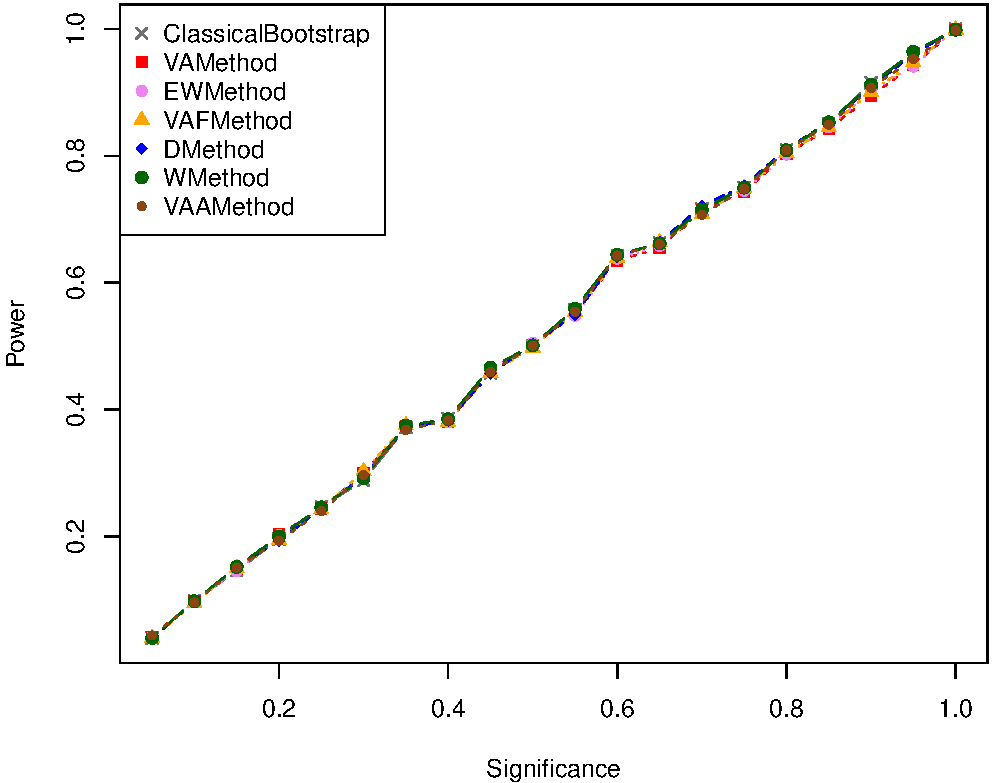
\includegraphics[scale=0.4]{size_plot_1_v2.pdf}
	\caption{Test size depending on the significance level for the one-sample C-test  based on the samples generated with \code{GeneratorNU}.}
	\label{fig1size}
	\end{minipage}  
\quad 
\begin{minipage}[b]{0.45\linewidth}
	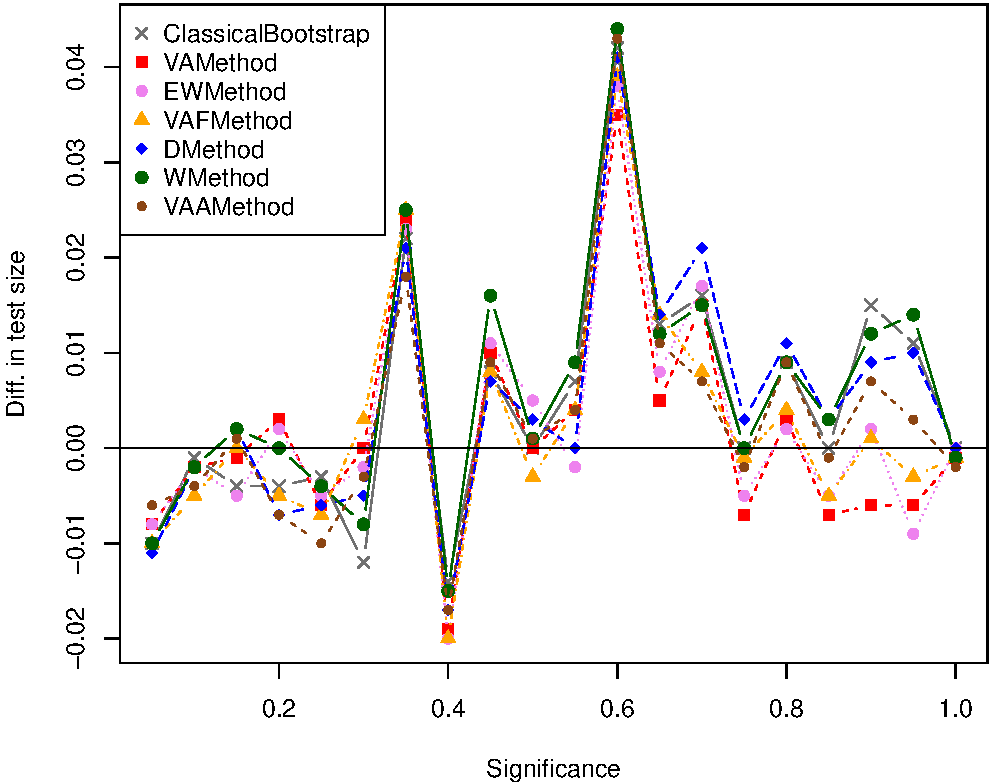
\includegraphics[scale=0.4]{size_plot_2_v2.pdf}
	\caption{Differences in test size between the resampling methods and the significance level.}
	\label{fig2size}
	\end{minipage}  
\end{figure}

Our experiments confirm the conclusion stated in \citep{grzegorzewski_amcs2020} that the classical bootstrap was never the winner in such comparisons. New resampling methods usually behave much better -- especially the $d$-method and the VA-method. The EW-method behaves always in a relatively stable manner and never drops below the third place.


%%%%%%%%%%%%%%%%%%%%%%%%%%%%%%%%%%%%%%%%%%%%%%%%%%%


\subsection{Test power analysis}


Our package also enables  the power comparison for the one-sample C-test combined with different resampling methods. This is possible by using the \code{ComparisonOneSampleCTest} function, which determines the percentage of the null hypothesis rejection under increasing shift added to the initial sample:
\begin{example}
ComparePowerOneSampleCTest (generator,mu_0,shiftVector,sampleSize = 10,
 numberOfSamples = 10,initialSamples = 100,theta = 1/3,significance = 0.05, ...)
\end{example}
This procedure produces a matrix with the successive shift values, set in the vector \code{shiftVector}, specified in the rows and the corresponding percentages of rejections for the respective resampling methods given in columns.

Below we show how to apply this function to comparisons based on very small samples  ($n=5$). To minimize undesired random effects the following experiment was repeated 10000 times:
\begin{example}
# prepare vector of shifts
> shifts <- seq(0.1,1,by = 0.05)

> set.seed(1234567)

> outputCPowerTest1 <- ComparePowerOneSampleCTest(generator="GeneratorNU",
+ mu_0 = c(-0.4,-0.1,0.1,0.4),shiftVector = shifts,sampleSize = 5,numberOfSamples = 100,
+ initialSamples = 10000,mu = 0,sigma = 1,a = 0.2,b = 0.6)

> head(round(outputCPowerTest1, digits = 4),4)

     ClassicalBootstrap VAMethod EWMethod VAFMethod DMethod WMethod VAAMethod
0.1              0.0274   0.0302   0.0305    0.0314  0.0288  0.0276    0.0278
0.15             0.0278   0.0321   0.0321    0.0305  0.0304  0.0293    0.0297
0.2              0.0315   0.0357   0.0337    0.0325  0.0339  0.0326    0.0302
0.25             0.0386   0.0393   0.0386    0.0391  0.0395  0.0397    0.0366
\end{example}
The results given both in the output matrix and in Fig.~\ref{fig1power} show that the new resampling methods have greater power than the classical bootstrap approach.
To better highlight the results, differences between the power curves for each of the new resampling methods and Efron's bootstrap are plotted in Fig. \ref{fig2power}.
Observing these results we can agree with the conclusions of simulations reported in \citep{GrzegorzewskiRom2021}, that ``In general (i.e. including other models) this method \emph{(VA-method)} was usually one of the best, especially for smaller sample sizes or a lower number of bootstrap replications (e.g.  $b=100$). The VAA-method or the EW-method were usually just after VA-method; the d-method, w- and the VAA-method were neither too good nor too bad, but the classical bootstrap (as compared with other resampling methods) was usually the worse method in hypotheses testing.''


\begin{figure}[htbp]
  \centering
	\begin{minipage}[b]{0.45\linewidth}
	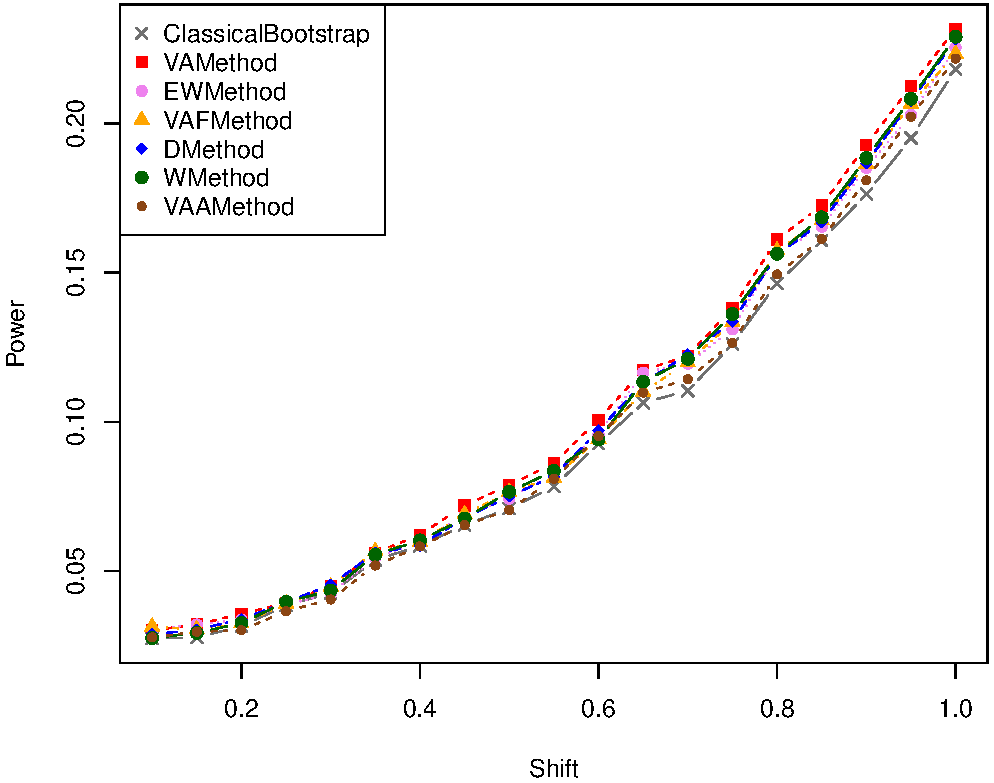
\includegraphics[scale=0.4]{power_plot_1_v3.pdf}
	\caption{Power curves of the one-sample C-test based on the samples generated with \code{GeneratorNU}.}
	\label{fig1power}
	\end{minipage}  
\quad
\begin{minipage}[b]{0.45\linewidth}
	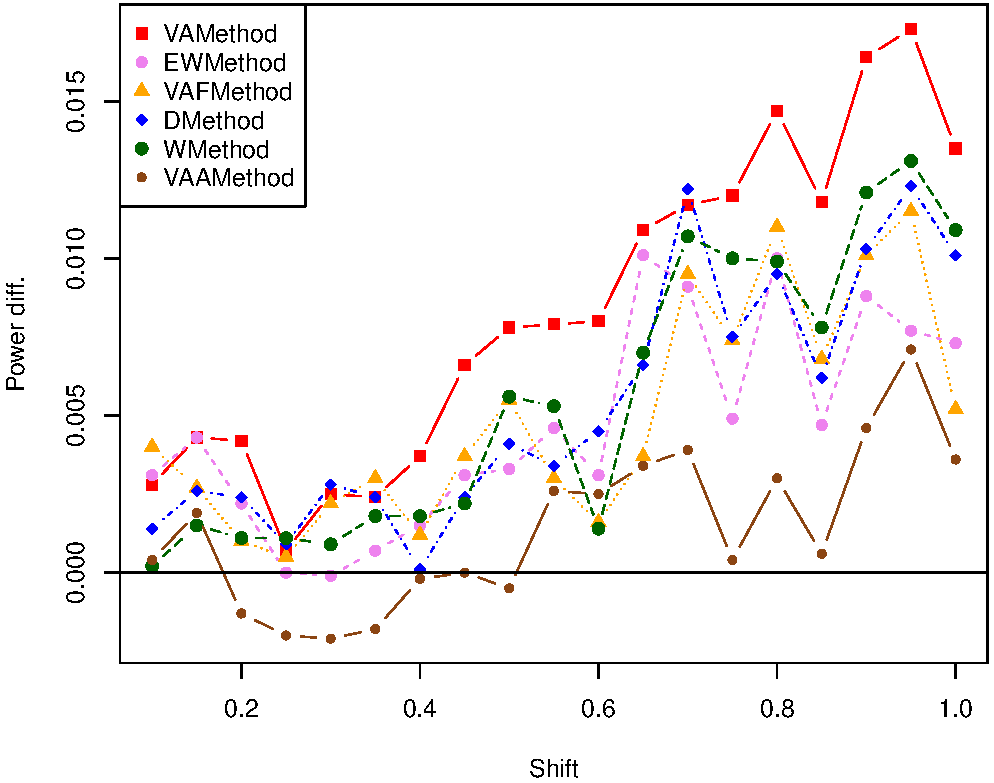
\includegraphics[scale=0.4]{power_plot_2_v3.pdf}
	\caption{Differences in power curves between the new resampling methods and the classical approach.}
	\label{fig2power}
	\end{minipage}  
\end{figure}


%%%%%%%%%%%%%%%%%%%%%%%%%%%%%%%%%%%%%%%%%%%%%%%%%%%


\subsection{Two-sample test -- a real-life case}

Finally, we compare the resampling methods combined with the two-sample C-test applied to some real-life imprecise data. Such data may appear naturally wherever we deal with expert opinions expressed in everyday language. In our study, we consider the opinions of the experts related to the Gamonedo cheese quality (a kind of blue cheese produced in Asturias, Spain). The inherently imprecise assessments were modeled by the TPFNs \citep{ramos2019}.

To check whether two given experts, say A and C, differ significantly in their opinions, we verify the null hypothesis \eqref{h0ctestc2} of no difference \citep{grzegorzewski_amcs2020}. We can perform the desired test using the following function based on \code{TwoSampleCTest}:
\begin{example}
CompareRealCaseTwoSample(numberOfSamples, numberOfIterations)
\end{example}
which delivers p-values of the two-sample C-test for all resampling methods.
To eliminate undesired randomness each experiment (i.e. the bootstrap procedure for the single test) is repeated \code{numberOfIterations} times and then the obtained p-values are averaged.
The parameter \code{numberOfSamples} is passed directly to \code{TwoSampleCTest}.

Then the following function is applied:
\begin{example}
> set.seed(1234567)
> realCaseP <- CompareRealCaseTwoSample(numberOfSamples=100,numberOfIterations=10000)
> 
> round(realCaseP,5)
     ClassicalBootstrap VAMethod EWMethod VAFMethod DMethod WMethod VAAMethod
     0.82055            0.91213  0.88388  0.85542   0.82179 0.82212 0.85455
\end{example}
Assuming any reasonable significance level, the null hypothesis $H_0$ is not rejected. Thus, whichever resampling method is applied, we may conclude that the given two experts do not differ significantly in their opinions.
However, the new resampling methods usually lead to greater p-values than the classical bootstrap (i.e. we are ``more sure'' that $H_0$ can be accepted).


%%%%%%%%%%%%%%%%%%%%%%%%%%%%%%%%%%%%%%%%%%%%%%%%%%%


\section{Conclusions}

The main goal of the proposed resampling algorithms for fuzzy samples of trapezoidal fuzzy numbers is to overcome the shortcomings typical to the classical bootstrap.
New approaches are implemented in \pkg{FuzzyResampling} package and are supplemented with some ready-to-use functions useful in statistical inference based on imprecise data.
It is shown that, in some cases analyzed in this paper and related literature, the suggested bootstrap algorithms are more effective than the classical one.

Obviously, many problems are still open. New methods and algorithms that would be helpful in solving many problems faced by practitioners are still needed. In particular, an in-depth study on the so-called ``epistemic bootstrap'' \citep{grzegorzewski2021} would be useful to handle ``epistemic data'' instead of the ``ontic data'' \citep{Couso2014} discussed in this paper.


%%%%%%%%%%%%%%%%%%%%%%%%%%%%%%%%%%%%%%%%%%%%%%%%%%%
  
\bibliography{fuzzyResampling}
  

  
  \address{Maciej Romaniuk\\
    Systems Research Institute, Polish Academy of Sciences\\
    Newelska 6, 01-447 Warsaw\\
    Poland\\
    (0000-0001-9649-396X)\\
    \email{mroman@ibspan.waw.pl}}
  
  \address{Przemys{\l}aw Grzegorzewski\\
    Faculty of Mathematics and Information Science, Warsaw University of Technology \\
    Koszykowa 75, 00-662 Warsaw\\
    Poland\\
    Systems Research Institute, Polish Academy of Sciences\\
        Newelska 6, 01-447 Warsaw\\
        Poland\\
    (0000-0002-5191-4123)\\
    \email{przemyslaw.grzegorzewski@pw.edu.pl}}
  
  

